\documentclass[UTF8,fontset=fandol,zihao=-4]{ctexart}
\usepackage[a4paper,margin=25mm]{geometry}
\usepackage{amsmath,amssymb,booktabs,array,graphicx,hyperref,xcolor}
\usepackage{caption,fancyhdr}
\hypersetup{colorlinks=true,linkcolor=blue,citecolor=blue,urlcolor=blue}
\setlength{\headheight}{15pt}
\setlength{\emergencystretch}{2em}
\pagestyle{fancy}\fancyhf{}\fancyhead[L]{ParallelBayes：补充材料}\fancyfoot[C]{\thepage}
\newcommand{\E}{\mathbb{E}}
\newcommand{\R}{\mathbb{R}}
\title{ParallelBayes：补充方法与完整历史核验记录}
\author{中文研究稿：作者与单位待定}
\date{2026 年 10 月}

\newcommand{\ind}{\mathbf{1}}
\begin{document}
\maketitle
\noindent 本材料保留历史实验的完整数值、诊断、成本口径、跨系统定位和安装记录。各节描述所属批次，不是当前紧凑研究的完成回执；当前正文按研究问题重新组织。原生成段落及其生成器保持不变，旧图表作为历史证据保留。正文新增的可读配对图不改变原始比值或区间。Windows端已完成紧凑研究交付，Mac端已接收全部证据，全目标统计重建仍在进行。本材料先加入已完成的数值失败和双峰原始路径伴随审查。
\setcounter{tocdepth}{1}\tableofcontents
\clearpage

\section{水井后验可正规化的充分条件}
仅有截距和距离系数两个参数，且平坦先验相对于$d\alpha\,d\beta$定义。保存数据的1基行号533/531在3.25200009346008米分别对应结局0/1；2884/190在151.065994262695米对应0/1。实际协变量为距离除以100，记两个不同值为$a,b$。设$g(v)=\sigma(v)\{1-\sigma(v)\}$，选取上述四个似然因子，其余因子均不超过1，故
\[
L(\alpha,\beta)\leq g(\alpha+a\beta)g(\alpha+b\beta).
\]
因为$\int_{\mathbb R}g(v)\,dv=1$且变量变换行列式绝对值为$|b-a|>0$，
\[
0<\int_{\mathbb R^2}L(\alpha,\beta)\,d\alpha\,d\beta
\leq\frac{1}{|b-a|}<\infty.
\]
因此该二维模型后验可正规化。归档证书使用较松的指数包络及$4/|b-a|$上界，同样有效，原件保留。此证明不认证数值求积参考的有限区域误差或稀有事件精度，也不直接适用于另加回归系数的模型。

\section{紧凑研究的原始路径伴随检查}
\subsection{内部停止与外部路径标准}
完整正式原件经分块和成员SHA校验后，另读取全部42项数值失败：quasi-DEER MALA在CPU/CUDA的1024预算各7项、4096预算各13项；顺序MALA在两设备的4096预算各1项。它们均来自中心化漏斗H1。候选输出的内部状态为完成，最终状态则由外部路径审计置为失败；状态链与原随机数组分别核对，没有重分类。

Mac使用冻结的独立NumPy递推、实际初值和输入数组复核602112次转移，42份仍全部越过原完整路径界限；接受事件计数均与保存输出一致。最大绝对路径差为$5.72867\times10^{-3}$，每项最严重链的误差/界限比在1.12至36238.48之间。quasi-DEER的40份候选均满足保存的局部归一化残差不超过1，不能据此推出全路径已达标。两份顺序失败也表明，这不是并行求解独有的数值现象。该补查重放被排除的确定递推，不新增采样或放宽标准；逐链数值和所有原失败数组保留。

\subsection{双峰符号事件与初始化}
事后伴随分析遍历M1全部432个任务，读取412份有效拟合的1648条链及初值、预热或丢弃段、保留段。穿越定义为相邻保存状态的$\mathbf1(q_1>0)$变化，零归入非正侧；不计算HMC积分器内部未保存的位置。路径符号与原函数二进制及四链均值逐项核对。20份失败NUTS拟合的部分链不进入完整拟合统计。

384份有效MH拟合没有保存状态的符号穿越；28份有效NUTS拟合中，原重复5、1024步CPU拟合的第三条链发生一次负侧到正侧穿越，该链保留段正侧比例为0.4599609375，四链合并比例为0.614990234375。其余411份拟合均无穿越，合并比例恰为0.5。全部实际初值均为两条负侧、两条正侧，因此零符号平方误差可以由均衡起点维持。

本文将它作为初始化与函数解释的边界，而不是宣称跨峰是每个后验函数估计正确的必要条件。已知权重下的模式分层估计需要自身的条件与不确定性规则。1648条链、不同工作流和两档预算也不是新增独立重复：原独立单位仍是每目标24份四链输入。正文图选择唯一穿越例及相同原重复的CPU顺序RWM，完整逐项结果另附。

\section{历史CPU验证与开发证据}
软件测试覆盖密度、梯度、Jacobian、约束输出、固定噪声路径、接受事件、拒绝自环、部分窗口、迭代耗尽、非有限目标、内存守卫和共同随机输入回退。错误注入包括遗漏 Jacobian、改变尺度以及改变实际目标造成接受事件失配。协议与文件校验测试还检查重复任务跳过和输出损坏检测。有限测试不能替代一般正确性证明，但提供了可重放的反例检测机制。

冻结0.1.0通过43项Python测试和R包检查。审查修订版0.1.1进一步通过58项Python检查、R包检查及R到BridgeStan的端到端核验；后者的固定输入样本差为零。CPU主实验仍对应归档的0.1.0，新版边界修复不覆盖历史输出。高斯、logistic 与正值模型的 Stan/原生实现交叉核验通过；两个简单高斯目标上，上游固定提交的求解器与独立 MALA 参考的路径差小于 $10^{-8}$。这项复现仅检验上游求解器与指定映射的组合，不声称复现原文全部性能实验。

开发探测使用 G1、G2、L1、L2，固定转移数为 256 或 2048，窗口为 16、64、256，每组采用三个实际随机输入数组。192 项任务均完成，最大路径差为 $2.17\times10^{-9}$。Mac CPU 上的并行执行通常增加了时间；尤其是大数据 logistic 的多次梯度与导数求值成本明显。该探测属于开发资料，最早若干任务与初次 Stan 编译重叠，因此不用于正式速度推断。

小型生成式校准检查从 $\theta\sim N(0,1)$ 及八个 $y_i\sim N(\theta,1)$ 生成 12 个独立数据集，每个数据集运行五种工作流。后验具有解析均值 $\sum_i y_i/9$ 和标准差 $1/3$。60 次拟合均完成，MALA 的顺序/并行秩直方图相同，RWM 的顺序/并行结果也相同。该重复数下，观察到的区间覆盖不能确证校准；秩抽样的相关性和有限功效须继续检查。正式 SBC 使用另一组 64 个生成数据集和独立种子，避免把已观察的开发样本作为未见验证资料。

在正式SBC拟合开始前，另冻结依赖数据的对数似然统计量 $f_y(\theta)=-\tfrac12\sum_i(y_i-\theta)^2$，并从同一批保存样本计算其秩和解析后验期望误差。秩每32步取一个样本，共64个；与真参数处统计量相等的样本单独计数，以独立Philox流在并列范围内随机化秩。此伴随分析不改变拟合协议，也不据有限、仍可能相关的秩宣布一般校准通过。

\section{历史Mac CPU的冻结实验设计}
\subsection{目标族与基线}
\begin{table}[htbp]\centering\small
\begin{tabular}{lll}\toprule
目标 & 定义 & 比较作用\\\midrule
G1 & 8 维标准高斯 & 简单几何与执行开销\\
G2 & 64 维旋转高斯，条件数 100 & 耦合与尺度差异\\
L1/L2 & 8 参数 logistic，样本量 256/4096 & 似然计算量\\
H1/H2 & 9 维漏斗，中心化/非中心化 & 相同分布的坐标与预热效应\\
A1 & 64 维潜在 AR(1) 高斯后验 & 高维相关结构\\
M1 & 8 维对称双峰高斯混合 & 跨模式探索压力\\\bottomrule
\end{tabular}
\caption{Mac CPU主协议的目标库。H1/H2 属于同一模型族；L1/L2 是同类回归的计算量变化。数据由记录的随机规则生成。本研究不把这些变体当作独立应用领域。}
\end{table}

五种工作流为顺序 MALA、窗口 quasi-DEER MALA、顺序 RWM、Online Picard RWM 和 BlackJAX NUTS。各工作流均采用四链；MH 使用预先固定步长，前 512 步作为丢弃段，随后保留 256 或 2048 步。NUTS 单独预热 512 步后保留相同数量，最大树深为 8。所有初始化固定为零，步长表、数据、随机种子及运行顺序写入机器可读协议。比较的对象是这些指定工作流，不能外推为经过全局最优调参的算法排名。

正式协议在独立探测后冻结，每组 24 次独立重复，共 1920 项任务。主实验不依据有利结果追加重复或选择模型。原研究计划提出的误差 MCSE 相对阈值 0.1 并未被承诺对每个压力目标满足；本版冻结有限重复数并完整报告其不确定性，区间跨阈值时保留为未判定。没有训练自动配置选择器，也没有将已见模型声明为选择器留出集。

\subsection{误差与参考}
对预先规定的函数集合 $\mathcal F$，以独立重复评价
\begin{equation}
 \widehat E_a(N)=\max_{f\in\mathcal F}\frac1R\sum_{r=1}^R
 \left(\widehat\mu_{a,f}^{(r)}(N)-\mu_f\right)^2/s_f^2.
\end{equation}
高斯目标使用标准化首坐标的均值、二阶矩及超过 1 的概率。漏斗目标使用标准化尺度变量、其双曲正切、局部变量的符号事件及条件标准化变量的余弦；这避免依赖漏斗局部变量的巨大高阶矩。双峰目标同时检查模式占比和连续函数。Logistic 检查前两个参数、截距的 logistic 变换及符号事件。全部函数与尺度在协议中明确，尺度统一取 1。

解析目标使用真实期望。L1/L2 的参考分别来自四次独立 NUTS 拟合，每次四链、预热 1024 步、保留 16384 步；参考种子与正式实验分离。两目标参考均未记录发散，L1的所检查函数及L2的连续函数 split-$\hat R$ 接近1，非退化函数参考MCSE最大约为 $7.6\times10^{-4}$。原协议计算所选函数的经典split-$\hat R$；审查后从相同保存样本补充秩正态化/折叠split-$\hat R$、bulk ESS和tail ESS，后文单列，不替换原分析。L2符号事件在全部参考样本中为零，其Rhat不可判定、参考误差未确定；不把零经验方差当作已证实的精度。参考 MCSE 取拟合间估计与批均值估计的较大值；该规则并不排除共同偏差。对这两个目标的结果称为参考平方差，不把它解释为无偏真实 MSE，也不无条件减去参考方差。

不确定性采用独立重复层面的 4000 次重采样，报告逐点 95\% 区间；每次重采样先在重复间求平方误差均值，再在预声明函数间取最大值。对可用共同参考另做正态、对角协方差扰动的敏感性传播，同一次扰动在所有重复中共用。它没有估计函数之间的完整参考协方差，不等于联合误差的精确传播；基本重复bootstrap区间另行保留。区间不是跨模型、方法和预算的同时置信保证。失败率、成功输出上的条件误差及全部成本分别呈现，有失败时不宣称无条件精度达标。

\subsection{计时与资源}
本地实验在 M4 Mac mini、16 GB 内存和 JAX CPU 后端上执行，使用 float64、JAX 0.6.2、BlackJAX 1.2.5、NumPy 2.2.6 和 BridgeStan 2.7.0。外层同一时刻运行一个实验任务。目标平台是整台指定机器，未将逻辑 CPU 个数直接解释为独占物理核预算。正式计算期间同机还进行了少量软件核验与文档生成，未实现全程独占空闲系统；保留全部原任务，不依据这种背景活动剔除计时值。

显式同步设备后结束执行计时。记录 JIT 编译、输入、NUTS 预热、执行、传输、独立核验和回退；逐任务墙钟还包含建模和写盘。本文以逐任务墙钟扣除额外计时重放成本、加上后验函数摘要与诊断计算时间，定义完整工作流时间；建模、原始数组写盘和校验和计算均在该口径内，另保留纯采样接口计时。完成初次执行后对同一编译程序进行两次缓存内重放，作为执行机制计时探测，额外成本单列；它们不是新的统计重复，也不计作增加后验样本。进程导入和一次性软件安装不是单次任务计时的一部分，因此本文不将该口径称为全新进程冷启动。

MH 的步长与窗口作为指定工作流的输入；开发探测属于离线研究费用，单独保留，不在每个正式拟合中重复摊入。NUTS 的逐次适配则包含在预热成本中。因此完整工作流比较回答的是给定配置的运行成本，尚未覆盖未知新模型上选择MH参数所需的成本，不应称为自动调参方案之间的完整费用比较。

CPU 内存为采样API期间每20 ms记录的进程绝对RSS峰值，包含先前驻留分配，未覆盖建模、写盘和子进程；该CPU协议不评价GPU内存；Windows另有设备分配器记录。数组空间有事前保守预算检查，数值迭代上限保留。运行没有人为总时长截止。冻结源代码和协议校验和、随机化任务顺序、逐任务原始数组与状态支持中断后恢复；成功与失败结果均保留。

\section{历史CPU结果与范围}
本机按冻结协议登记了 1920 项正式任务，全部结束，其中 0 项未返回满足输出标准的正常样本。失败计数与原始输出均保留；该总任务数包含配对执行，并非 1920 个独立模型。每个模型、预算及工作流的独立重复数为 24。

正常输出中，独立核验记录的最大数值路径差为 $2.36\times10^{-8}$，接受事件失配总数为 0。这一陈述以数值核验及当前目标库为边界，不构成一般轨迹或平稳分布证明。

quasi-DEER MALA 的模型—预算组中位缓存执行速度比范围为 0.0192 至 0.174，研究审计工作流速度比范围为 0.0715 至 0.739。速度比定义为同核顺序时间除以并行时间，小于 1 表示并行执行更慢；这里只统计成对有效输出，失败另行报告。

Online Picard RWM 的模型—预算组中位缓存执行速度比范围为 0.0503 至 0.809，研究审计工作流速度比范围为 0.226 至 0.814。速度比定义为同核顺序时间除以并行时间，小于 1 表示并行执行更慢；这里只统计成对有效输出，失败另行报告。

\begin{figure}[htbp]\centering
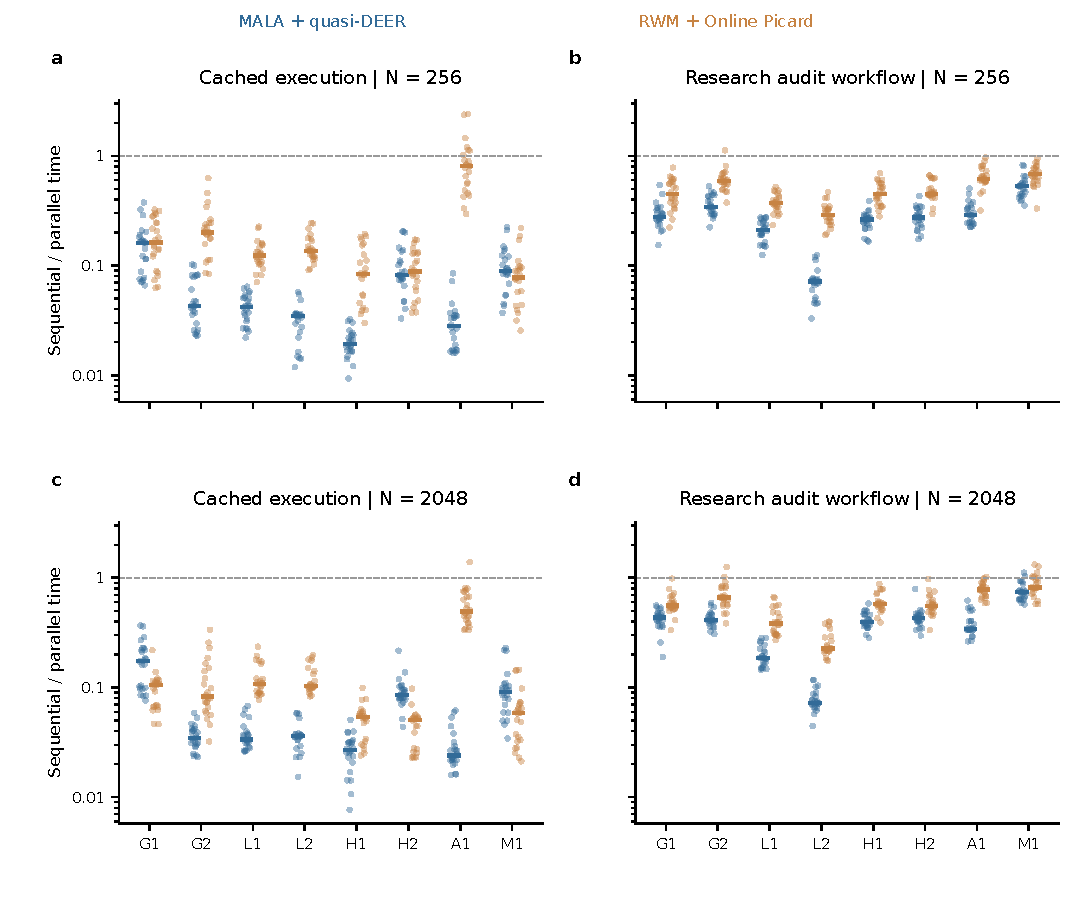
\includegraphics[width=\linewidth]{../../figures/software/paired-costs.pdf}
\caption{同核成对成本。上、下行分别为每链保留256和2048步；左列为两次缓存重放时间的中位数之比，右列为含编译、预热/丢弃段和独立核验的工作流时间比。每个点为一个独立重复中的配对比，短线为组中位数；同一轨迹的计时重放不当作统计重复。虚线表示速度比1。任何缺失配对均在原始任务及失败表中保留。}
\end{figure}

表中列出较大预算下的函数最大平方误差。L1/L2 采用有限参考，因此相应数值是参考平方差。完整逐函数误差、逐点区间、参考敏感性区间、失败比例区间及两预算结果随机器可读材料交付。不能把表中的最小数值自动解释为确定排名。

\begin{table}[htbp]\centering\small\setlength{\tabcolsep}{3pt}\begin{tabular}{lrrrrr}\toprule

目标 & 顺序MALA & quasi-DEER & 顺序RWM & Picard & NUTS\\\midrule

G1 & $0.00199$ (0) & $0.00199$ (0) & $0.00542$ (0) & $0.00542$ (0) & $0.000531$ (0)\\

G2 & $0.125$ (0) & $0.125$ (0) & $0.164$ (0) & $0.164$ (0) & $0.000322$ (0)\\

L1 & $0.000255$ (0) & $0.000255$ (0) & $0.000673$ (0) & $0.000673$ (0) & $1.46\times10^{-5}$ (0)\\

L2 & $6.22\times10^{-6}$ $\dagger$ (0) & $6.22\times10^{-6}$ $\dagger$ (0) & $1.91\times10^{-5}$ $\dagger$ (0) & $1.91\times10^{-5}$ $\dagger$ (0) & $2.28\times10^{-7}$ $\dagger$ (0)\\

H1 & $0.138$ (0) & $0.138$ (0) & $0.131$ (0) & $0.131$ (0) & $0.112$ (0)\\

H2 & $0.0215$ (0) & $0.0215$ (0) & $0.0376$ (0) & $0.0376$ (0) & $6.11\times10^{-5}$ (0)\\

A1 & $0.00803$ (0) & $0.00803$ (0) & $0.856$ (0) & $0.856$ (0) & $0.000665$ (0)\\

M1 & $0.252$ (0) & $0.252$ (0) & $0.359$ (0) & $0.359$ (0) & $0.296$ (0)\\

\bottomrule\end{tabular}\caption{每链保留2048步时的最大函数平方误差/参考平方差。括号内为该组24次重复中的输出失败数；有失败时，误差仅描述成功输出。误差不包含失败的假定损失，不代表无条件达标。$\dagger$表示参考精度未确定，该行仅展示参考平方差，不能判断全函数精度达标。}\end{table}

按前述工作流口径汇总，正式尝试合计耗时 5080.9 秒，其中失败任务耗时 0.0 秒。另有缓存计时重放开销5711.5秒，完整保留但不重复计入单次工作流成本。逐组成本及全部失败分母另存分析结果。

NUTS 在 46 个已返回有限样本的任务中记录到发散，总计 2358 个保留转移的发散事件。发散与数值输出失败分别呈现，不能因为数组有限而删除这一诊断。多峰和漏斗目标上的误差须结合模式占比及尺度函数理解。

NUTS另有6861个保留转移达到255个积分步的设定上限；积分步数及逐次适配参数随原始记录保存。

采样接口期间记录的逐任务进程RSS峰值范围为244.3至549.0 MiB；它包含进程已驻留内存，只覆盖接口调用阶段，不能解释为每种算法的独占增量内存或整项任务的严格峰值。

quasi-DEER的模型—预算组中，单个输出转移对应的前向转移映射求值次数中位数范围为14.58至66.15，顺序MH为1。

Online Picard的模型—预算组中，单个输出转移对应的前向转移映射求值次数中位数范围为2.00至21.38，顺序MH为1。

这些程序层面的映射调用计数包含丢弃段和拒绝自环，尚不包含独立审计；它们不是浮点运算量或密度/梯度调用次数。quasi-DEER的JVP另存，因此不能仅据调用数精确分解运行瓶颈。

\begin{figure}[htbp]\centering
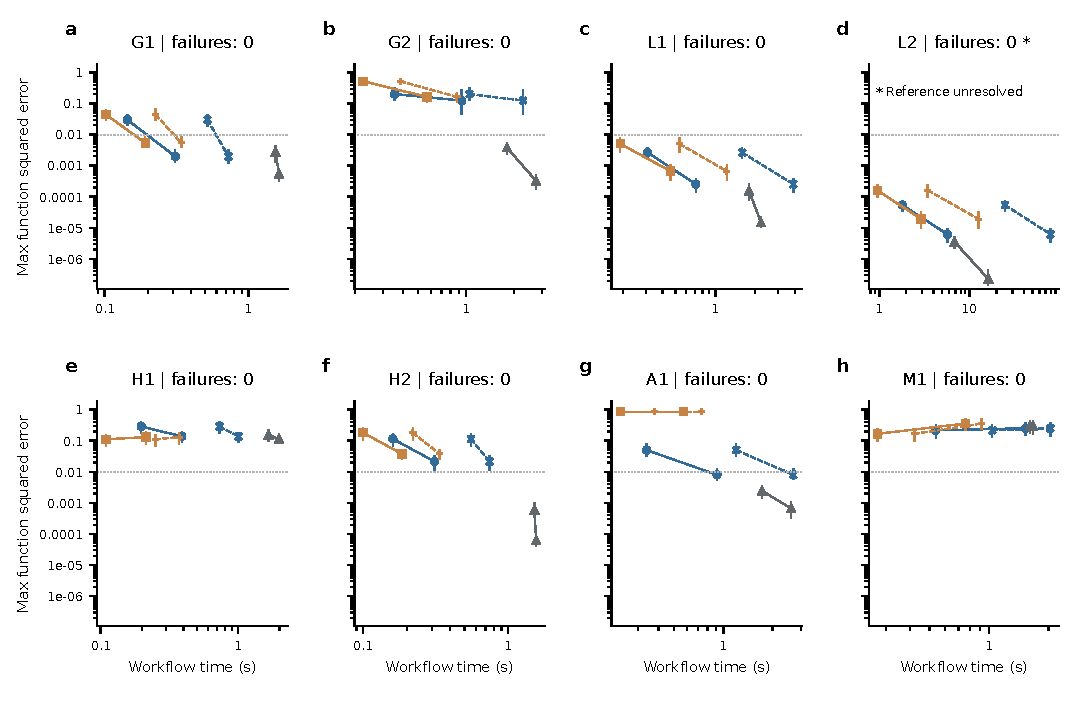
\includegraphics[width=\linewidth]{../../figures/software/error-cost.pdf}
\caption{固定采样计划的误差—成本关系。横轴为成功输出条件下的工作流时间中位数，全部尝试和失败成本另表保存。每条线连接同一指定工作流的两个预算点，不表示中间预算已被测量。蓝色为MALA、橙色为RWM、灰色为NUTS；实线/圆或方形为顺序MH，虚线/叉号为相应时间执行器，三角形为NUTS。误差取预声明函数中最大的重复平均平方误差；L1/L2为有限参考平方差。线段区间为逐点95\%重复重采样区间，有限参考的共同误差敏感性另行传播；传播采用正态对角协方差工作假设，非同时保证。星号表示参考精度未确定，该面板仅供探索性平方差比较。面板标题列出该模型全部正式任务中的输出失败数，失败组的误差为条件结果。点虚线标出0.01作为预声明误差阈值。}
\end{figure}

\noindent mala/sequential在较长预算、$\epsilon=0.1$下的逐点判断为：区间低于阈值2个目标，区间高于阈值4个，跨阈值1个，参考或输出条件不足1个。\par

\noindent mala/quasi\_deer在较长预算、$\epsilon=0.1$下的逐点判断为：区间低于阈值2个目标，区间高于阈值4个，跨阈值1个，参考或输出条件不足1个。\par

\noindent rwm/sequential在较长预算、$\epsilon=0.1$下的逐点判断为：区间低于阈值2个目标，区间高于阈值5个，跨阈值0个，参考或输出条件不足1个。\par

\noindent rwm/online\_picard在较长预算、$\epsilon=0.1$下的逐点判断为：区间低于阈值2个目标，区间高于阈值5个，跨阈值0个，参考或输出条件不足1个。\par

\noindent nuts/sequential在较长预算、$\epsilon=0.1$下的逐点判断为：区间低于阈值5个目标，区间高于阈值2个，跨阈值0个，参考或输出条件不足1个。\par

这些判断仅对应两个已测量预算中的较长预算，不构成同时置信结论，也不提供单次运行可观测的停止规则或精确的达标时间。

正式生成式检查完成64个新数据集、五种工作流，共320次拟合，其中0次输出失败。90\%后验区间的覆盖估计及其二项区间按数据集作为独立单位报告；保留所有秩与原始样本。抽稀秩仍可能相关，这一检查不提供一般SBC一致性证明。

\noindent mala/sequential：覆盖率 0.844，95\%二项区间 [0.731, 0.922]。\par

\noindent mala/quasi\_deer：覆盖率 0.844，95\%二项区间 [0.731, 0.922]。\par

\noindent rwm/sequential：覆盖率 0.828，95\%二项区间 [0.713, 0.911]。\par

\noindent rwm/online\_picard：覆盖率 0.828，95\%二项区间 [0.713, 0.911]。\par

\noindent nuts/sequential：覆盖率 0.828，95\%二项区间 [0.713, 0.911]。\par

正式生成式检查另记录到0个保留转移的发散事件，涉及0次拟合；该诊断与输出失败分开保存。

本次覆盖率点估计均低于名义90\%，而相应二项区间均包含90\%。这一有限重复结果既不能证明完全校准，也不应被改写为已确证系统性覆盖不足。

对数似然测试量也完成320次拟合的伴随分析，共记录0个秩并列。逐方法秩直方图、抽稀后相关性及解析期望误差随原始数据交付；这些描述性诊断不构成统一性检验或正确性证书。

L2 的参考符号事件在262144个相关样本中均为零，Rhat 对该函数不可判定，不能把零经验方差当作事件概率已被精确确定。因此保留原函数集合，并将L2全函数精度判定标记为未确定。没有通过删除该函数得到达标结论。

上述结果来自历史Mac CPU协议，不包含后续Windows实验；原生Windows实现及其独立协议的实测结果在后文另行报告。


\section{审查后的伴随分析与CPU机制实验}
\subsection{版本与扩展验证}
CPU主实验保留0.1.0源代码和原协议；0.1.1增加约束输出检查、末窗口有效步掩码、错误及失败记录，并修复R单元素数组。变换检查和掩码可能影响计时，不能用旧性能代表新版。审查后对8目标、5工作流各取原较短预算的第一个重复，旧/新源码分别执行；MH复用保存的实际随机数组，NUTS复用锁定随机流。40组均返回有效输出，最大路径差为$1.99\times10^{-13}$，接受事件零失配。这是有限数值对照，不是性能等价或边界正确性证明。

新增Poisson回归示例无需改动内核，公开模型对象分别实现JAX密度与独立NumPy密度/解析梯度，先验证坐标和导数，再比较固定输入的四种MH工作流。密度与梯度最大差约$2.84\times10^{-14}$；MALA和RWM配对最大路径差分别为$7.90\times10^{-11}$和$3.61\times10^{-16}$，接受事件无失配。示例旨在说明扩展和核验，不作为新性能或后验收敛证据。

\subsection{同数据集的解析SBC对照}
本节为审查后伴随分析，未追溯为原协议预声明检验。64组真参数和数据已保存，后验为$N(\sum_j y_j/9,1/9)$，故直接计算解析90\%区间，无需新增拟合。解析区间覆盖54/64，点估计0.84375，95\%二项区间为[0.731,0.922]。五种工作流共享同64组数据，同核顺序/并行还共享轨迹，因此不能当作五次独立校准证据。

\begin{table}[htbp]\centering\small\setlength{\tabcolsep}{4pt}
\begin{tabular}{lrrrrrr}\toprule
工作流 & 覆盖数 & 分歧数 & 下端点RMSE & 上端点RMSE & 均值RMSE & 标准差RMSE\\\midrule

顺序MALA & 54 & 4 & 0.0179 & 0.0195 & 0.0105 & 0.0063\\

quasi-DEER & 54 & 4 & 0.0179 & 0.0195 & 0.0105 & 0.0063\\

顺序RWM & 53 & 3 & 0.0318 & 0.0267 & 0.0147 & 0.0107\\

Picard & 53 & 3 & 0.0318 & 0.0267 & 0.0147 & 0.0107\\

NUTS & 53 & 3 & 0.0222 & 0.0190 & 0.0115 & 0.0078\\

\bottomrule\end{tabular}
\caption{同64数据集的配对解析对照。RMSE按数据集计算；分歧指解析与MCMC区间对同一真参数的覆盖判断不同，不能只据总体覆盖率相等判定区间相等。}
\end{table}
MALA的分歧数据集编号为23、32、36、56，RWM为26、32、56，NUTS为11、26、36（从0编号）。例如MALA有2例解析覆盖而MCMC未覆盖、另2例相反，抵消后总覆盖数相同。该批解析覆盖本身偏低，与有限生成样本波动的解释相容；端点及后验矩误差仍显示有限链估计差异，不能据此证明无额外采样偏差。

\subsection{现代诊断与有限预算误差的对应}
从全部1920项保存样本及8次参考拟合提取每个参数和预声明函数，以posterior 1.7.0计算秩正态化/折叠split-$\hat R$、bulk ESS与tail ESS\cite{posterior}。每个拟合分别计算，结果不替换原经典函数诊断；常量链等不可判定值保留为空。表中汇总NUTS，全80组的逐拟合、逐变量诊断随复现材料交付。

\begin{table}[htbp]\centering\scriptsize
\begin{tabular}{lrrrrrrl}\toprule
目标/$N$ & 发散\% & 上限\% & 最大$\hat R$ & 最小bulk ESS & 最小tail ESS & 函数误差 & 判据\\\midrule

A1/256 & 0.00 & 0.00 & 1.018 & 496.4 & 469.7 & 0.00243 & 低于阈值\\

A1/2048 & 0.00 & 0.00 & 1.002 & 5576.0 & 5186.4 & 0.000665 & 低于阈值\\

G1/256 & 0.00 & 0.00 & 1.018 & 1198.4 & 461.8 & 0.00271 & 低于阈值\\

G1/2048 & 0.00 & 0.00 & 1.003 & 11148.1 & 5316.6 & 0.000531 & 低于阈值\\

G2/256 & 0.00 & 0.00 & 1.015 & 636.5 & 448.0 & 0.00383 & 低于阈值\\

G2/2048 & 0.00 & 0.00 & 1.002 & 5848.5 & 5429.4 & 0.000322 & 低于阈值\\

H1/256 & 0.71 & 2.67 & 1.745 & 6.3 & 8.0 & 0.154 & 高于阈值\\

H1/2048 & 1.11 & 3.16 & 1.273 & 11.4 & 5.4 & 0.112 & 高于阈值\\

H2/256 & 0.00 & 0.00 & 1.018 & 815.5 & 545.5 & 0.000595 & 低于阈值\\

H2/2048 & 0.00 & 0.00 & 1.002 & 7125.8 & 5438.9 & 6.11e-05 & 低于阈值\\

L1/256 & 0.00 & 0.00 & 1.017 & 358.2 & 393.2 & 0.000154 & 低于阈值\\

L1/2048 & 0.00 & 0.00 & 1.003 & 3459.7 & 4381.6 & 1.46e-05 & 低于阈值\\

L2/256 & 0.00 & 0.00 & 1.019 & 507.4 & 532.0 & 3.52e-06 & 不可判定\\

L2/2048 & 0.00 & 0.00 & 1.002 & 4243.8 & 5109.4 & 2.28e-07 & 不可判定\\

M1/256 & 0.00 & 0.00 & 1.738 & 6.2 & 30.6 & 0.301 & 高于阈值\\

M1/2048 & 0.00 & 0.00 & 1.734 & 6.1 & 26.8 & 0.296 & 高于阈值\\

\bottomrule\end{tabular}
\caption{NUTS按模型和保留预算分组的伴随诊断。发散和上限命中以24次拟合、各4链的全部保留转移为分母；$\hat R$为参数与拟合中的最大值，ESS为最小值。函数误差为原预声明最大平方误差/参考平方差，判据对应原逐点95\%区间与0.01阈值，不由诊断阈值重定义。}
\end{table}
2358次发散与6861次积分上限命中均来自中心化漏斗H1：短/长预算分别为174/2184次发散及657/6204次上限命中。双峰M1无发散，却在两个预算下都有约1.73的最大参数$\hat R$，所选函数误差亦高于阈值。五个目标的长预算函数误差区间低于阈值，与H1/M1的探索问题分别成立；L2参数诊断良好不消除参考符号事件恒零的不确定性。特定函数误差小、无发散和后验全面探索是不同陈述。

\subsection{三种成本口径}
缓存执行衡量已编译内核；正常推断应包含必要建模、编译、预热、转换及诊断；研究审计另加入独立顺序参考和完整数组、校验和归档。历史时钟未单独测量正常输出与所有建模步骤，故只能以$T_{\rm API}-T_{\rm independent}+T_{\rm diagnostic}$给出内存内正常使用的记账估计，不能冒称重新实测的完整正常工作流。该估计不含未分离的建模、R转换和持久化费用。

\begin{table}[htbp]\centering\small\setlength{\tabcolsep}{4pt}
\begin{tabular}{lrrr}\toprule
执行器 & 缓存执行 & 正常内存口径估计 & 研究审计工作流\\\midrule

quasi-DEER & 0.019--0.174 & 0.038--0.175 & 0.072--0.739\\

Picard & 0.050--0.809 & 0.110--0.393 & 0.226--0.814\\

\bottomrule\end{tabular}
\caption{历史主实验中，各模型--预算组的配对速度比中位数范围。三列均为顺序时间/并行时间；中列是不同包含项的记账敏感性分析，不与另外两列混称三种完整实测工作流。}
\end{table}
共享审计成本使速度比向1靠近，可能掩盖加速或减速；当前缓存与去独立核验的估计口径也均未显示组中位加速，因此负结果不能仅归因于审计。新增机制实验另直接计量\texttt{audit=False}的建模、采样与基本均值/方差/链间诊断，并单列普通样本输出耗时；它是最小Python正常工作流，不包含R转换及现代posterior诊断，也不是全新进程冷启动。

\subsection{小型CPU机制实验}
审查后另冻结\texttt{cpu-mechanism-v1}，使用0.1.1，目标G1/G2/L1、链数1/4、窗口16/64、每链256步、两组成对MH执行方式和每格3个新实际随机数组，共72项任务。沿用主协议的指定核参数，冻结随机顺序；没有按速度追加或删除任务。每次至少7次缓存计时重放、总观测窗口至少0.2秒，作为技术重复而非独立统计重复。全部72项完成；分段重放与生产程序首链的接受事件无失配。

生产执行另外记录进程CPU秒/墙钟秒和10毫秒间隔系统利用率。组中位进程占用约为1.00--2.99个CPU核当量，测量包含运行返回和监测开销，不是物理核心绑定，也不能将\texttt{vmap}当作指定核心数的证明。固定前驱状态的微基准比较串行映射与向量化映射在同一批状态、噪声上的吞吐；它没有MCMC的递推依赖，不能将吞吐比直接当作轨迹加速比。

\begin{figure}[htbp]\centering
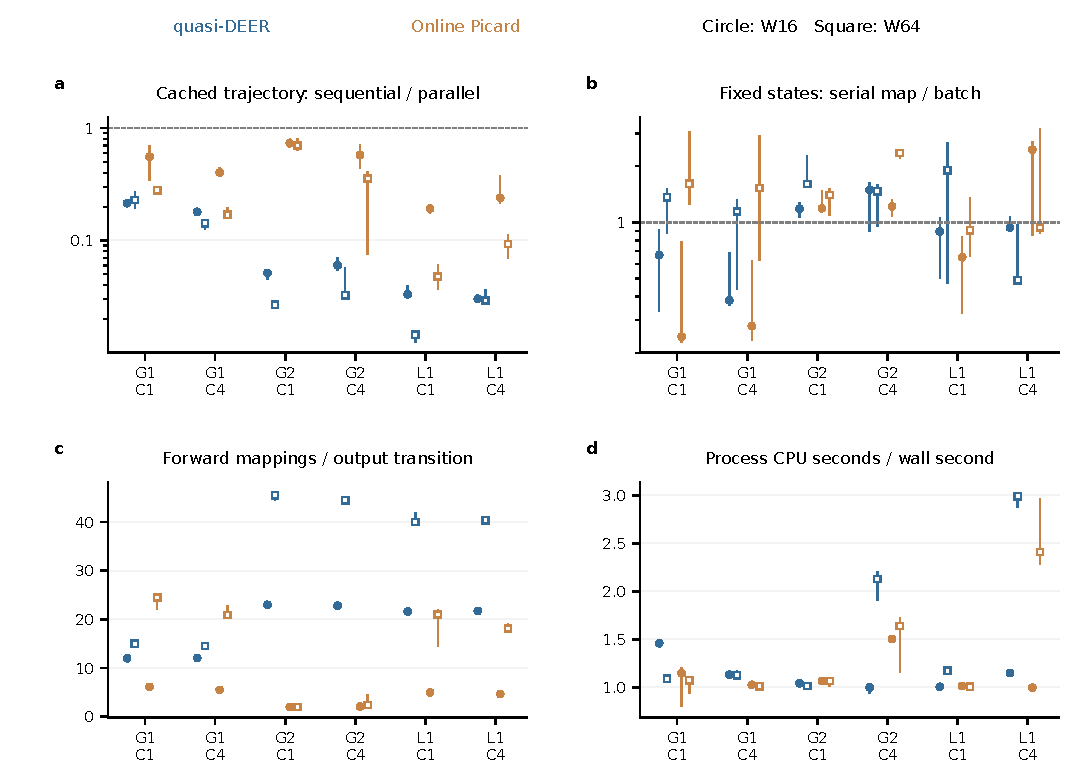
\includegraphics[width=\linewidth]{../../figures/software/cpu-mechanism.pdf}
\caption{新冻结的72项机制任务。每格3个实际随机数组，符号为组中位数，细线为最小至最大值；技术计时重复不扩大样本量。蓝色为quasi-DEER，橙色为Picard；圆点为窗口16，方形为64；横轴C为链数。a：缓存轨迹速度比，1以上才为加速。b：固定状态批量吞吐比，1以上表示批处理有利，但它不是轨迹加速。c：每个输出转移的前向映射求值数，quasi-DEER还另有JVP；拒绝自环计入转移。d：进程CPU秒/墙钟秒，表示观测消费量而非核数配置。}
\end{figure}

quasi-DEER的组中位缓存速度比为0.0145--0.23，固定状态批量吞吐比为0.381--1.91；每转移前向映射数为12--45.5，另有5.5--22.2次JVP。

Picard的组中位缓存速度比为0.0477--0.732，固定状态批量吞吐比为0.244--2.46；每转移前向映射数为2--24.5。

这些量显示局部批量求值收益与完整轨迹重复工作之间的差距，而非证明单一瓶颈。例如G1、四链Picard把窗口从16增至64时，首链每轮确认数的组中位数均约5.57，前向工作却从5.50增至20.88次/转移，缓存速度比由0.402降至0.170。G2、单链quasi-DEER的平均每窗口轮数由11增至22.25，前向工作从23增至45.5次/转移，速度比由0.051降至0.027。窗口扩大会增加可批处理宽度，但确认推进和求解轮数决定有效工作效率；这些例子是冻结小网格中的观察，尚未识别正加速的交叉点。

为审查阶段组成，另将首链实现拆成单独编译的批量求值/JVP、扫描和接受复核，并记录每轮残差或确认前缀。拆分插入同步及Python控制，改变了融合执行。所得控制及未细分部分比例很高，不能据此宣称生产程序主要受Python控制限制；它暴露了分段探针的扰动。全部阶段秒数和原始逐轮记录公开，可用于复查数值过程；对生产程序的精确XLA剖面仍属于局限。三次独立重复及短微基准不足以给出普遍硬件因果结论。

\subsection{可移植复现检查}
另建锁定依赖的Python环境并安装非editable轮子，在迁移目录运行完整测试。首次57项通过、1项因漏带上游比较源文件而失败；补齐许可与该源文件后，仅复查失败项并通过，保留初次失败日志。迁移目录的新目标示例也通过。R包检查日志与显式\texttt{PB\_RUN\_INTEGRATION=1}的3项集成测试日志分别交付，后者实际执行15个断言，不以默认跳过替代通过。

迁移目录从1920项主实验、8次参考拟合和320项SBC原始证据重建主摘要，逐字节一致。三个归档含全部源代码、协议、原始数组和论文输入；新临时目录解压后，校验、分析、1928项现代诊断重算、绘图和编译均通过，诊断值排除耗时后逐项一致。检查仍共享Mac、R库和编译器，不等同外部团队或异构系统复现。



% Data source: benchmark/analysis/outputs/windows-native-v1/delivery-review.json
% Scientific source: 0c9325e98f2bc7dcd75d344c01c2e50a62801c90
% Protocol identity: 1d233dd09956c4575fc5775082310e5edca65407db5fcef40bc2ce329e6f5898
% This companion fragment has not been compiled into a revised PDF on Windows.
\section{原生Windows扩展：独立开发版本与新冻结实验}
\label{sec:windows-native}

开发分支\texttt{windows-native-dev}新增Python版本0.2.0.dev1及R版本0.2.0.9001。
明确torch目标与独立NumPy参考可在不导入JAX的条件下运行，基础安装不再强制拉取JAX。
本轮实际环境为Windows 11、AMD Ryzen 7 9800X3D、NVIDIA RTX 5080（sm\_120）、
驱动616.56、Python 3.12.14、torch 2.13.0+cu130及float64。
R 4.6.1通过reticulate整批调用并保持iteration$\times$chain$\times$variable次序。
Stan仍为CPU提供方式，未自动翻译；本轮未编译核验原生Stan。
Pyro 1.9.2的CPU NUTS仅作为单独正态目标统计基线，未接入GPU NUTS。

实现保持相同MALA/RWM核约定、硬接受前向、独立参考与实际随机数组。
quasi-DEER使用非重叠窗口和截断Rademacher对角JVP；Picard使用滑动窗口，
多链按最小已确认前缀共同推进，末窗口只处理实际转移。
控制采用torch eager与Python循环，记录主机标量等待，不宣称融合设备内控制。
CPU 65项和CUDA 63项测试通过，另有72项原始路径比较与8个R批量核验。
这些有限测试不构成一般正确性证明。

试探网格96项完成后，在观察正式结果前冻结\texttt{windows-native-v1}。
协议包含8个目标、128/512两个预算、每组4份独立随机数组、CPU/CUDA资源和4个MH工作流，共512项，
每项4链、窗口16。新身份同时锁定源码、依赖、设备、数据、数组、坐标、函数与失败规则。
所有512项通过数值输出检查，接受事件对独立NumPy参考零失配，最大路径差为$5.212\times10^{-10}$。
256对CPU/CUDA实际数组比较亦无事件失配，最大无约束及约束差分别为
$2.842\times10^{-14}$及$5.684\times10^{-13}$。未发生回退或终结失败。

\begin{table}[htbp]\centering\small
\begin{tabular}{lrr}\toprule
资源 & quasi-DEER/MALA & Online Picard/RWM\\\midrule
CPU & 0.101--0.359 & 0.774--3.560\\
CUDA & 0.164--0.505 & 1.097--5.230\\\bottomrule
\end{tabular}
\caption{同设备、同torch、同核的warmed执行速度比（顺序秒数/时间执行器秒数）：
各16个模型/预算组中位数的最小至最大值。两次技术重放不增加独立重复数。
这不是GPU相对CPU的速度比，也不是精确达标时间。}
\end{table}

\begin{figure}[htbp]\centering
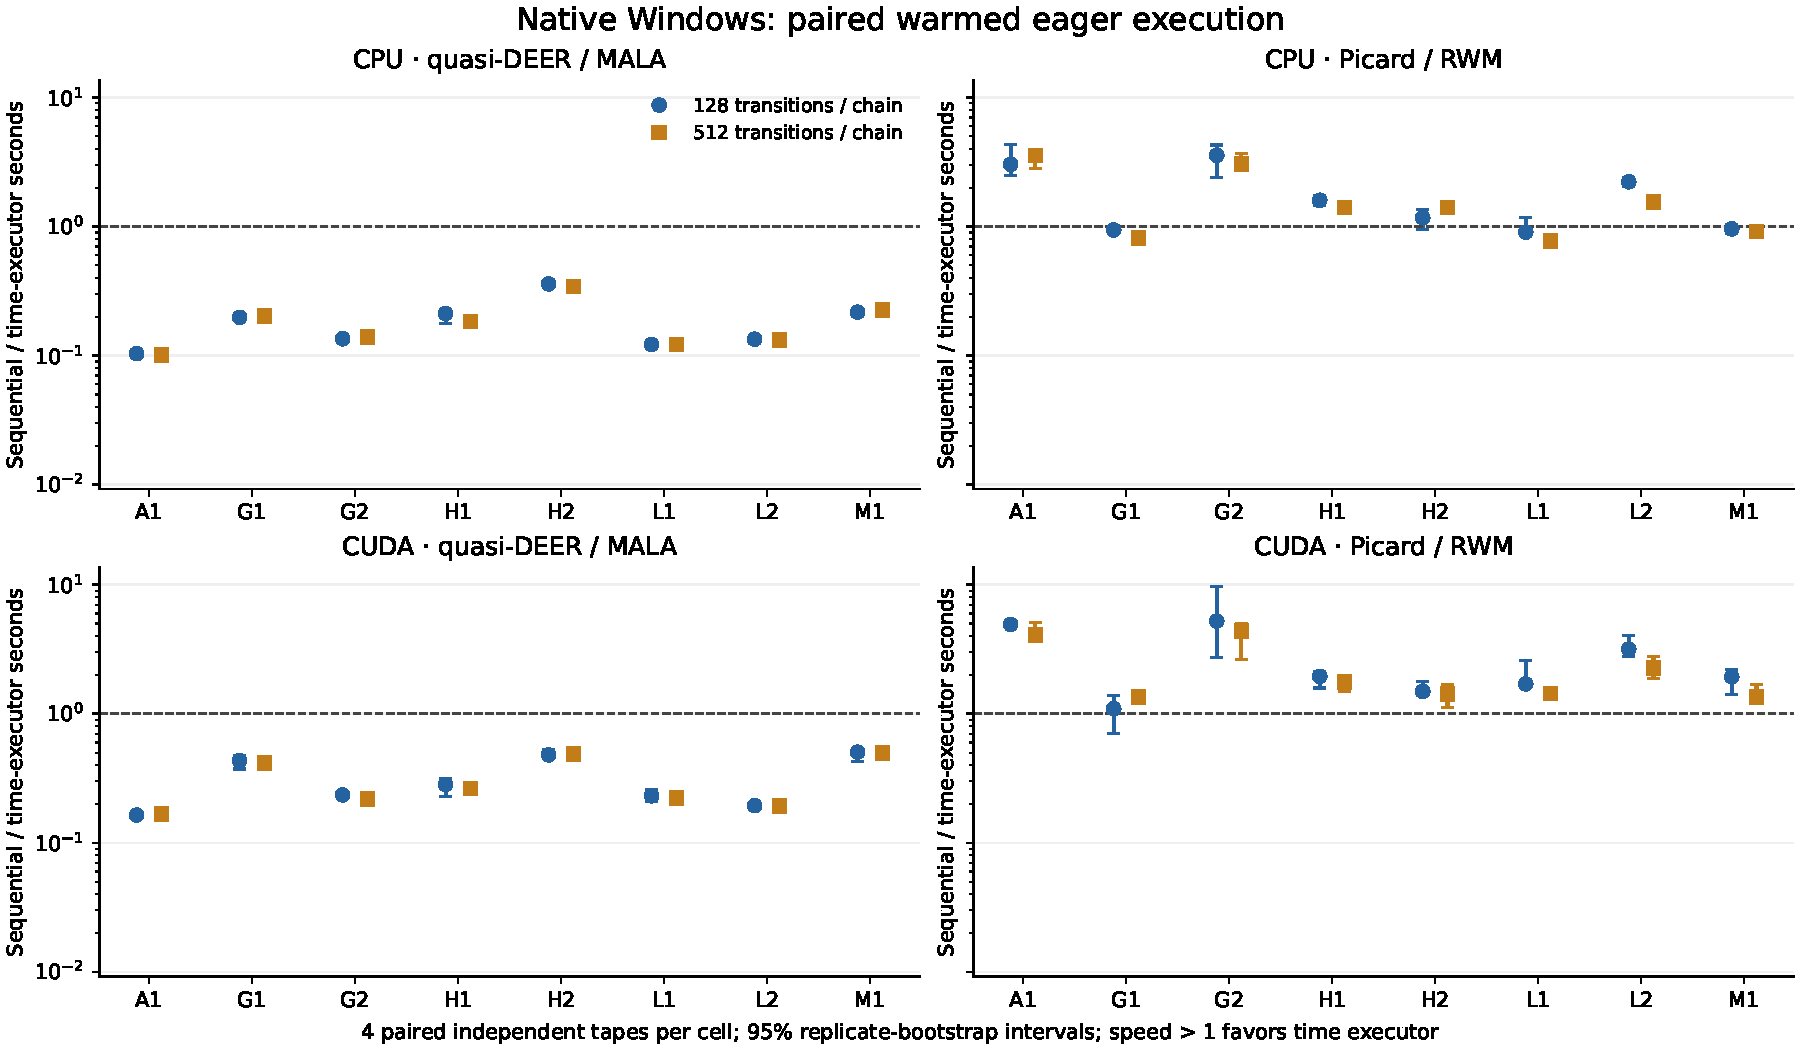
\includegraphics[width=\linewidth]{../../benchmark/analysis/outputs/windows-native-v1/speed-ratios.pdf}
\caption{原生Windows配对执行结果；每组4份独立数组，误差线为重复层面2000次bootstrap的逐点95\%区间，
不提供同时置信保证。CUDA Picard的16组中位数大于1，其中15组区间下限大于1。
A1/RWM的全部32次拟合均拒绝所有提议，其速度仅反映自环执行，不能解释为后验探索加速。
quasi-DEER的所有组中位速度比均小于1；全部负结果保留。}
\end{figure}

数值完成与推断可靠性有明显区别：480/512次拟合至少有一个有限rank/folded Rhat大于1.01，
108次拟合包含常量变量或函数，其诊断保留为不可判定。
最大有限Rhat为4.666，最小有限bulk/tail ESS为4.085/4.205。
该Rhat计数仅为描述，没有新增事后验收标准。解析目标的逐函数重复MSE及区间另行保存；
L1/L2的有限参考未解决，不宣称精度达标。全拒绝或混合不足轨迹没有被删除或重新调参替换。

另以12个新生成数据集进行小型SBC，五个共享数据工作流共60次拟合全部完成。
同数据解析90\%区间与五个工作流的覆盖均为9/12，解析覆盖的95\%区间为[0.428,0.945]；
端点、矩和诊断分别保存。共享数据不能计作60个独立校准重复。
Pyro CPU NUTS与MH不使用固定同轨迹比较，也未纳入本轮正式速度实验。

正式任务记录成本共1790.220秒（含普通执行和技术重放），现代R诊断另计28.470秒；
普通API、核验API、写盘和诊断分开计时，不能混称完整工作流。
最大CUDA分配/保留峰值为97,251,328/115,343,360字节，包含已有驻留分配；
CPU仅有数组空间估算，未测逐拟合RSS峰值。主机标量读取累计88,406次，
标量等待计时4.206秒含设备等待，并不隔离全部控制开销。
试探分析曾把共享数组的配置变化合并为误差区间；该区间已撤回，原输出及哈希保留，正式分析不受影响。
本轮结果仅支持指定Windows实现和有限预算下的计算证据，不将Mac JAX与Windows torch的完整工作流差异全部归因于GPU。

% Reviewed input SHA256 d8b3a6090148f1ea7d3d49c20bb01d2349b345e5c1fab5d0c209021fb0f17e4e benchmark/protocols/mechanism-windows-pilot-v1.json
% Reviewed input SHA256 c99b15bf200d78d57b25faf668de37d7fb0c04cfd9c2729640fb6798859f1772 benchmark/analysis/outputs/windows-followup-intake-v1/comparison-summary.json
% Reviewed input SHA256 8b89658b151fa4a0852038f497e6838edaf18da3409b56b7f199b86827f87a37 benchmark/analysis/outputs/windows-followup-intake-v1/numpy-summary.json
% Reviewed input SHA256 d4b9ce12c23ecdbff615bc6566e2a5a61e43cf073aeadbb7f193bd82db670f86 benchmark/analysis/outputs/windows-followup-intake-v1/runtime/SUMMARY.json
% Reviewed input SHA256 1d3576fe927db1433c2712f5caaff45c24aacaf6401527068754323feeda0ffa manuscript/software/intake.generated.tex
% Reviewed input SHA256 749f6f6710211b9cde823f13f051db57e45ad6b9a1c59d5cb3f9766b9f449f9e manuscript/software/followup.template.tex
% Reviewed input SHA256 cb5bc9c51a9735d5e7f7a10de697c141ecac47093c26c6de5d505042a7b29329 figures/windows-mechanism-pilot-v1/work-and-cached-cost.pdf
% Reviewed input SHA256 04d86adde990daa6809994ed97b0cbd3fb81a940771a5f0e6a54101b02134c7f benchmark/analysis/outputs/mechanism-windows-pilot-v1/windows-20261006/analysis-cpu/workflows.csv
% Reviewed input SHA256 9e2fd3b87f61bbb453aac19b038c42bbe11710d5d2ff455239b5ffafe48c4b8b benchmark/analysis/outputs/mechanism-windows-pilot-v1/windows-20261006/analysis-cuda/workflows.csv
% Input SHA256 c34ec98f0093c93effb5a37fbaeb8c8739b1d7f5ad263825e3272317a047eaec benchmark/analysis/outputs/windows-round2-intake-v1/summary.json
第二轮接收把无约束路径、参数变换与下游诊断分别核对。
108份MH保存路径均在原容差内，接受事件失配为0；但从同一无约束状态在Mac重算原尺度输出时，
60份不满足原逐位相等要求，最大绝对差为$8.88\times10^{-15}$。
这项严格跨系统检查仍记为失败，不能通过事后添加容差改称全部通过。
Windows同机核验与Mac跨系统重算回答不同问题。

CPU Pyro NUTS在9个目标上的串行/四进程技术对照中，54组保存数组逐字节相同。
对收到的18份原二进制重新计算R诊断，有限$\hat R$与tail ESS一致，
bulk ESS最大差约$1.02\times10^{-12}$，不可判定位置一致。
这不意味着重复计算后验函数也必然逐位相同，更不增加独立统计重复数。
原短链的探索不足仍然成立。

实际数组传递同样是复现契约的一部分。第二轮启动时，Windows重新生成的六份候选输入中，噪声与导数探测数组相同，但对数均匀数组有82/49152个元素不同，最大差约$4.44\times10^{-16}$，因此原协议拒绝启动机制工作流。随后传递原始封存文件，按原哈希和容差完成了下述测量；原启动失败与候选数组仍保留。相同种子和依赖版本不能替代实际数组校验，核验本身也未确定底层数学库差异的因果来源。

\subsection{Windows有限机制测量}
独立机制协议在G1、G2、L1上各使用2份主随机输入，比较窗口4/16、链数分配及预先规定的G2 RWM步长对照。CPU与CUDA各完成96个工作流；每个工作流包括首次审计、3次交错缓存重放和探针后重放。全部960份保存路径通过独立NumPy参考核验，接受事件零失配，最大绝对路径差为$3.84\times10^{-10}$。技术重放、窗口变体和跨设备副本均不增加独立输入数。

测量使用同一台Windows 11计算机的Ryzen 7 9800X3D和RTX 5080，torch主机线程设为4，CUDA使用float64并显式同步。桌面显示负载仍存在，不将线程数等同独占物理核心数。表\ref{tab:windows-mechanism}给出全部配置的描述性比值；它们来自三次缓存sample时间中位数之比，既不是完整推断成本比，也不是跨独立重复的置信区间。

\begin{table}[htbp]\centering\small
\begin{tabular}{lrrl}\toprule
设备/执行器 & 配对数 & 比值大于1 & 全部比值范围\\\midrule
CPU / quasi-DEER & 24 & 0 & 0.092--0.322 \\
CPU / Picard & 36 & 20 & 0.612--3.574 \\
CUDA / quasi-DEER & 24 & 0 & 0.139--0.437 \\
CUDA / Picard & 36 & 32 & 0.778--4.805 \\
\bottomrule\end{tabular}
\caption{机制协议的同核缓存执行比值：同组顺序时间除以时间执行器时间。全部120个时间执行配置均保留；quasi-DEER对应MALA，Picard对应RWM。每模型仅两份独立输入，配对数不能解释为独立实验数。}
\label{tab:windows-mechanism}
\end{table}

quasi-DEER每个输出转移对应7.75--22.5次前向映射及3.875--11.25次JVP；Picard为2--7.59375次前向映射（图\ref{fig:windows-mechanism}）。这些计数包括拒绝自环，均高于顺序执行的一次前向映射；映射与JVP不是等价浮点工作量，不能简单相加。每端6个工作流完全零接受，全部保留。例如G2/RWM步长1.0的第一份输入，在窗口4/16下可一次确认整个窗口，同时没有接受移动。因此较长的确认前缀可以由自环产生，并不表示更有效的后验探索。

\begin{figure}[htbp]\centering
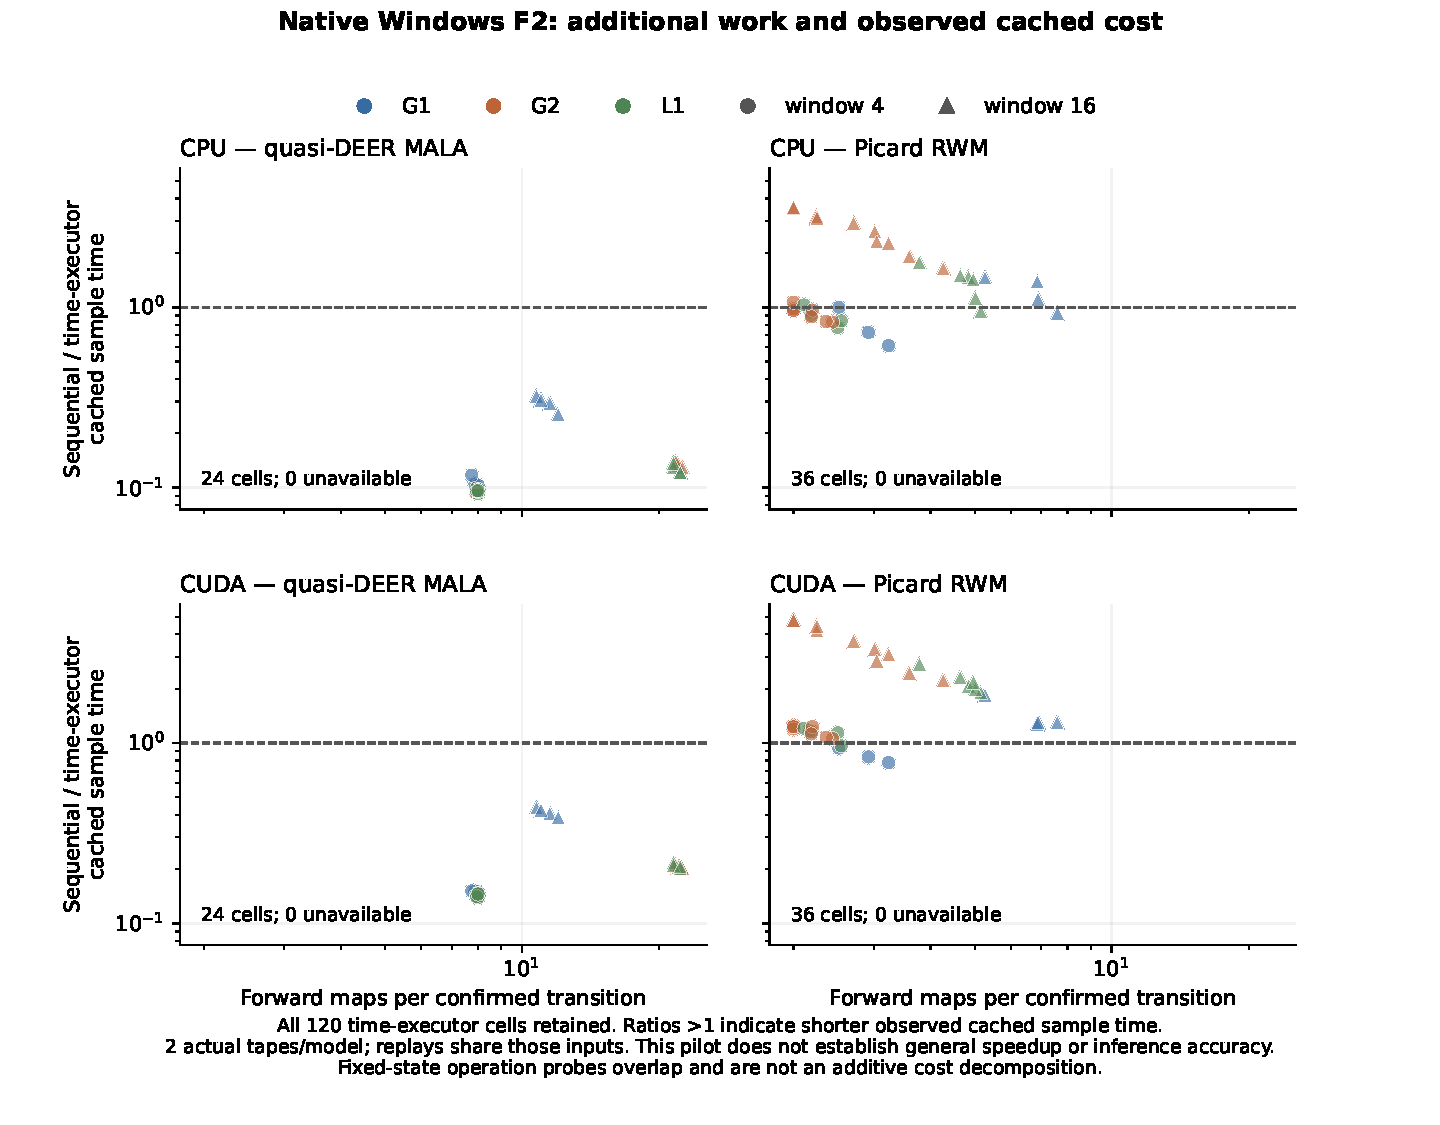
\includegraphics[width=\linewidth]{../../figures/windows-mechanism-pilot-v1/work-and-cached-cost.pdf}
\caption{Windows机制测量中的重复求值与缓存成本。每点为一个配置与实际输入的组合，共120点，部分重叠；颜色区分目标，点形区分窗口。上下行为CPU/CUDA，左右列为quasi-DEER/Picard。纵轴大于1表示指定缓存执行较短；横轴包括拒绝自环。三次技术重放不扩充独立样本量，图中没有推断精度或统计区间。操作探针存在重叠，不用于构造可加的独占耗时分解。}
\label{fig:windows-mechanism}
\end{figure}

预先规定的等512个总输出对照提供了另一种解释边界。在G2、L1的两份输入及两个设备上，16条各32步的顺序链均比单条512步、窗口16的Picard链更快，后者时间为前者的4.43--6.92倍。这8个技术对照说明链数分配会改变执行吞吐；两种分配的轨迹长度、初始化份数及探索能力不同，不能解释为相同推断精度下的优劣。图示的额外工作量与quasi-DEER减速相容，但不足以唯一归因于JVP、扫描或主机控制；固定状态操作探针与生产路径不同，同步及嵌套操作也使各阶段不能相加还原总时间。

\subsection{批次运行与安装的实测范围}
另一个Windows技术批次完成27项主任务和24项缓存探测（96次调用），包含最大形状、进程集合管理和终态恢复检查。接收端对保存MH数组独立重放，并核对函数与R诊断；这没有新增正式推断重复。90条函数诊断中仍有59条$\hat R>1.01$及27条tail ESS不可判定，不能将运行成功解释为收敛。该批次支持其封存运行器的技术能力；后续正式协议适配器的独立Windows验收与充分预算比较仍需完成。

Python 0.2.0.dev2与R 0.2.0.9002候选已在Windows新建依赖环境和仓库外完成安装核验，覆盖CPU/CUDA MH和R批量入口。默认R包检查与显式集成测试分别保存；成功检查不隐去此前安装和locale失败。接收端核对源码、sdist、wheel与R包中17个模块，并从保存RDS重建诊断，没有在Mac重新测量CUDA。该证据不涵盖原生Windows的JAX/Stan安装、GPU NUTS或第三方团队的独立复现。

% Reviewed input SHA256 9b9341f765e1c43252db0a6cf6289b95bd90de21d8d49dc1d6bb5c09d95600e8 benchmark/analysis/outputs/windows-formal-v2-intake-v1/receiver-summary.json
% Reviewed input SHA256 2bf882cae2e3710549ad21588fe8a22292cc3b63ef85ef038b56139d48ce4ca5 benchmark/analysis/outputs/windows-formal-v2-intake-v1/analysis-resume-summary.json
% Reviewed input SHA256 04c47765f64c30796f278a574650f320dd86c0dbdd27afb9f77ec6f3e04bb65a benchmark/analysis/outputs/windows-formal-v2-intake-v1/source-design-bridge.json
% Reviewed input SHA256 d7a22eee1795d966e663ae3f3399f43a17c27b737717df95cdf56f2c734a258a benchmark/analysis/outputs/windows-formal-v2-intake-v1/G1/diagnostics.csv
% Reviewed input SHA256 d8902be4286adc9386a8314431846c424602e60f0d82893ed02a0800eb00826d benchmark/analysis/outputs/windows-formal-v2-intake-v1/G2/diagnostics.csv
% Reviewed input SHA256 97d5222a0f5188bb17327e3e6d7bd1895dd8b17af2e3b89686132e23f3eba9f9 benchmark/analysis/outputs/windows-formal-v2-intake-v1/W1/diagnostics.csv
% Reviewed input SHA256 af07ce8044628c2bb8e4521732cd8248eea3b79f129f90c70fafadcfb2066cbc manuscript/software/adapter.template.tex
\subsection{原生适配与独立接收的验证层次}
\label{sec:native-adapter-validation}
任务执行、证据归档和统计解释分别接受核验。独立冻结的原生适配验收在G1、G2和水井W1各使用一份实际输入，运行27项四链主任务及24项缓存探测；G1/W1每链保留64步，G2保留16384步。接受原生进程、故障隔离、恢复和身份拒绝检查后，主任务全部返回数值合格结果，缓存96次调用仍无普通后验样本资格。前期句柄及测试环境失败、失败测试尝试与修复记录一并归档，没有将测试重试计为新的科学拟合。

接收端在Mac上按完整任务表重读原始证据，对24项MH主工作流及全部缓存调用独立重放NumPy递推，接受事件失配均为0；三项CPU NUTS按数组、随机状态、适应记录和子进程证据核对，不作MH同路径声明。随后从原始函数二进制重建全部117条R诊断，按既定跨平台输出条件通过比较；这与早期要求原尺度输出逐位相等的检查是不同契约，没有将此前60份严格变换失败改为通过。恢复分析复用51项结果，未重新采样或重算诊断，原始文件不变。

数值合格仍不能解释为后验探索充分：本次117条函数记录中，83条有限$\hat R$大于1.01，9条$\hat R$及27条tail ESS不可判定。这些记录共享每个目标的一份输入，不能据工作流或缓存调用数建立正式独立重复区间。逐函数诊断、跨平台末位差、数值库警告及原生故障链见配套接收报告；当前证据支持该固定适配版本的有限运行与接收能力，九目标多预算的正式推断比较仍未冻结或执行。


\subsection{外部目标与测量接口}
水井案例采用posteriordb的3020个观测，保留原模型中截距和距离系数的平坦先验，而非用带正态先验的内置logistic替代。通过两个不同距离上均出现两种结局的观测，可构造可积的似然上界；本数据的后验因而可正规化。Stan、NumPy和torch的密度及导数对照、固定输入轨迹与R数组传输已核验，Windows的12项接口工作流也已独立重放。这些是目标和软件扩展证据；短链的明显不良诊断仍保留。有限参考样本与数值求积另行核对，未认证的罕见事件概率不能改写成解析真值。该案例已用于开发，不能再作为未见模型族的泛化检验。

后续充分预算比较需要将可用输出和完整成本对应到同一批重复。为此，已实现三种分别记录的测量口径：准备后、显式同步的内核执行；包含进程启动、输入读取、采样、变换、普通输出与R诊断的批量工作流；以及进一步包含独立轨迹参考、资源检查和封存的研究审计调用。后两者为嵌套边界，不能相加。给定核参数和已封存输入的普通工作流不包含事先调参、环境安装或最外层R前端；这些费用须另列。后续终态核验也独立登记，不因增加检查次数而改变第一次推断的成本。

一次完整四链拟合是重复单位，链、缓存重放和基础设施重试不增加重复数。任何一次实际尝试缺少计时回执时，该任务的完整成本保持未知，已知部分仍保留。对函数$f$，误差和成本坐标使用同一组数值有效且函数估计有限的重复；其中任何任务缺完整成本，不能通过删去它来生成横坐标。函数不可计算、参考未确定、数值失败和基础设施中断分别记录。共同可用重复上的成对费用比与误差差也采用同一集合，避免混合不同条件样本。

上述归并与统计接口已连接有限原生适配批次的实际证据；完整任务表、缓存资格、跨系统函数诊断及零重算恢复均有接收回执。该方法准备没有追溯替换历史CPU或Windows首轮的计时与bootstrap规则，也不为尚未执行的正式推断提供结果。


\clearpage
\section{首轮Windows的CPU配对点}
\begin{figure}[htbp]\centering
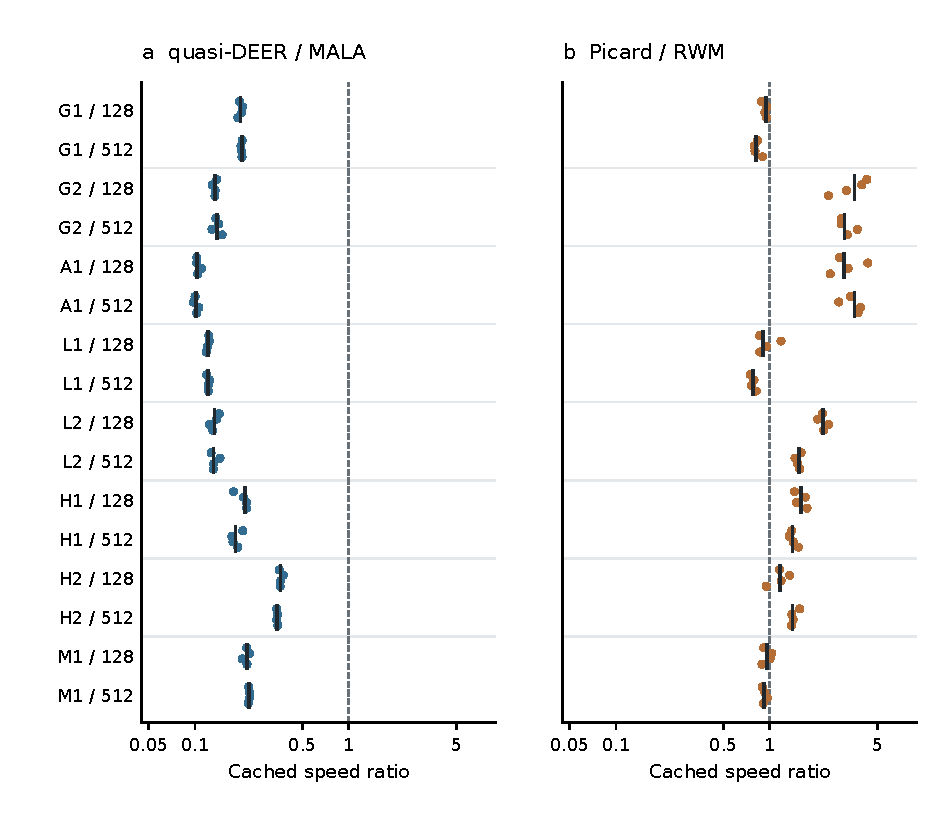
\includegraphics[width=\linewidth]{../../figures/software-revision/windows-cpu-pairs.pdf}
\caption{首轮Windows CPU全部配对输入的缓存速度比。四个点为每格四份实际数组；黑色短线为中位数，不作置信区间。两个面板依次对应quasi-DEER MALA与Picard RWM。}
\end{figure}
\clearpage
\begin{thebibliography}{99}\small\setlength{\itemsep}{2pt}
\bibitem{zoltowski} Zoltowski D.M., Wu S., Gonzalez X., et al. \href{https://proceedings.nips.cc/paper_files/paper/2025/hash/202886ee1c9ca735cb5bff3a00a69883-Abstract-Conference.html}{Parallelizing MCMC Across the Sequence Length}. Advances in Neural Information Processing Systems, 2025, 38.
\bibitem{grazzi} Grazzi S., Zanella G. \href{https://doi.org/10.1093/biomet/asag022}{Parallel computations for Metropolis Markov chains with Picard maps}. Biometrika, 2026, 113(2): asag022.
\bibitem{stan} Carpenter B., Gelman A., Hoffman M.D., et al. \href{https://doi.org/10.18637/jss.v076.i01}{Stan: A Probabilistic Programming Language}. Journal of Statistical Software, 2017, 76(1): 1--32.
\bibitem{bridgestan} Roualdes E.A., Ward B., Carpenter B., Seyboldt A., Axen S.D. \href{https://doi.org/10.21105/joss.05236}{BridgeStan: Efficient in-memory access to the methods of a Stan model}. Journal of Open Source Software, 2023, 8(87):5236.
\bibitem{blackjax} Cabezas A., Corenflos A., Lao J., Louf R., et al. \href{https://arxiv.org/abs/2402.10797}{BlackJAX: Composable Bayesian inference in JAX}. arXiv:2402.10797, 2024.
\bibitem{pyro} Bingham E., Chen J.P., Jankowiak M., et al. \href{https://jmlr.org/papers/v20/18-403.html}{Pyro: Deep Universal Probabilistic Programming}. Journal of Machine Learning Research, 2019, 20(28):1--6.
\bibitem{comparemcmcs} NIMBLE development team. \href{https://github.com/nimble-dev/compareMCMCs}{compareMCMCs: Tools for comparing MCMC efficiency from NIMBLE and other engines}. 软件作者仓库，访问于2026年10月3日。
\bibitem{pplbench} Kulkarni S., Shah K.D., Arora N., et al. \href{https://arxiv.org/abs/2010.08886v1}{PPL Bench: Evaluation Framework For Probabilistic Programming Languages}. arXiv:2010.08886v1, 2020. 软件来源：\url{https://github.com/facebookresearch/pplbench}。
\bibitem{posteriordb} Magnusson M., Torgander J., Bürkner P.-C., Zhang L., Carpenter B., Vehtari A. \href{https://proceedings.mlr.press/v258/magnusson25a.html}{posteriordb: Testing, Benchmarking and Developing Bayesian Inference Algorithms}. Proceedings of Machine Learning Research, 2025, 258:1198--1206.
\bibitem{posterior} Stan development team. \href{https://mc-stan.org/posterior/reference/rhat.html}{posterior: Rhat, bulk ESS and tail ESS documentation}. 软件文档，版本1.7.0。
\bibitem{parallelmcmc} Senne R. and contributors. \href{https://github.com/rsenne/ParallelMCMC.jl/tree/7be9c866c8be03ad994a5e7f0486ec3290088813}{ParallelMCMC.jl}. 软件仓库，提交7be9c86，访问于2026年10月6日。
\bibitem{bayesforge} Sosa S. \href{https://cran.r-universe.dev/BayesForge/doc/manual.html}{BayesForge: Bayesian Inference using numpyro and XLA}. R包0.0.1参考手册，访问于2026年10月6日。
\bibitem{meads} Hoffman M.D., Sountsov P. \href{https://proceedings.mlr.press/v151/hoffman22a.html}{Tuning-Free Generalized Hamiltonian Monte Carlo}. Proceedings of Machine Learning Research, 2022, 151:7799--7813.
\bibitem{laps} Robnik J., Seljak U. \href{https://proceedings.mlr.press/v300/robnik26a.html}{Faster Parallel MCMC: Metropolis Adjustment Is Best Served Warm}. Proceedings of Machine Learning Research, 2026, 300:2719--2727.
\bibitem{fsm} Dance H., Glaser P., Orbanz P., Adams R.P. \href{https://proceedings.mlr.press/v267/dance25a.html}{Efficiently Vectorized MCMC on Modern Accelerators}. Proceedings of Machine Learning Research, 2025, 267:12436--12458.

\bibitem{gonzalez} Gonzalez X., Warrington A., Smith J.T.H., Linderman S.W. \href{https://arxiv.org/abs/2407.19115v3}{Towards Scalable and Stable Parallelization of Nonlinear RNNs}. arXiv:2407.19115v3, 2025（初版2024）.
\bibitem{vehtari} Vehtari A., Gelman A., Simpson D., Carpenter B., Bürkner P.-C. \href{https://doi.org/10.1214/20-BA1221}{Rank-Normalization, Folding, and Localization: An Improved R-hat for Assessing Convergence of MCMC}. Bayesian Analysis, 2021, 16(2):667--718.
\bibitem{modrak} Modrák M., Moon A.H., Kim S., et al. \href{https://doi.org/10.1214/23-BA1404}{Simulation-Based Calibration Checking for Bayesian Computation: The Choice of Test Quantities Shapes Sensitivity}. Bayesian Analysis, 2025, 20(2):461--488. DOI:10.1214/23-BA1404.
\bibitem{owen} Owen A.B. \href{https://artowen.su.domains/mc/}{Monte Carlo theory, methods and examples}. 2013, Chapter 9: Importance sampling. 在线书稿。
\end{thebibliography}

\end{document}
